\documentclass{report}
\usepackage{caption}
\usepackage{amsmath}
\usepackage{amssymb}
\usepackage{amsthm}
\usepackage{graphicx}
\usepackage{multirow}
\usepackage{geometry}
\usepackage{listings}
\geometry{a4paper,scale=0.8}

\begin{document}

\section*{question 1.}
\par In the example 1.1, we can know that the objective function 
is 
\begin{align*}
    f'(x)=(130c-2-2cx)e^{cx}-0.45.
\end{align*}

Then we can use One-Variable Newton's Method to solve this optimal problem. 
We can find the sensitivity of $x$ to $c$.

\begin{table}[htbp]
    \centering
    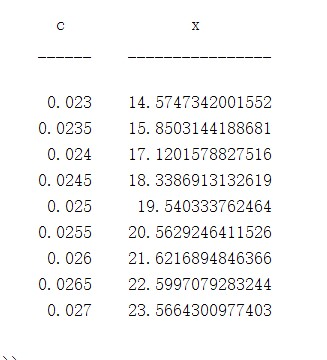
\includegraphics[scale=0.8]{figs/1_1.jpg}
    \caption{Sensitivity of best time to sell x to growth rate parameter c for the pig problem with nonlinear weight model.}
\end{table}

Next is the codes to achieve the result using MATLAB\@. 

\begin{figure}[htbp]
    \centering
    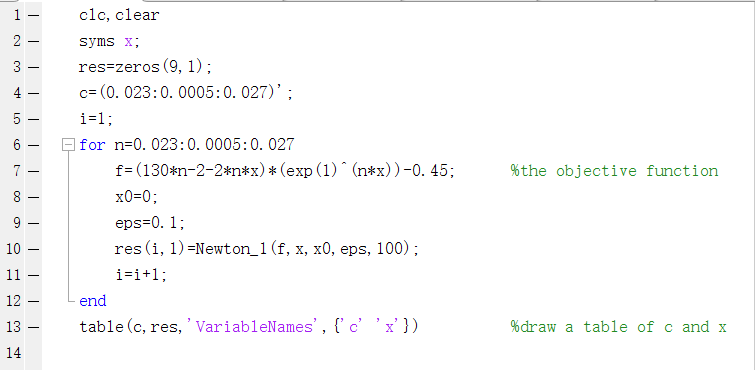
\includegraphics[scale=0.8]{figs/1_2.jpg}
    \caption{Main codes 1 in MATLAB}
\end{figure}

\begin{figure}[htbp]
    \centering
    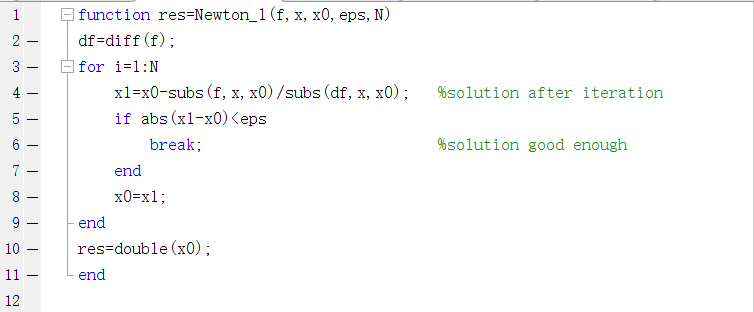
\includegraphics[scale=0.9]{figs/1_3.jpg}
    \caption{Function codes 1 in MATLAB}
\end{figure}

\newpage
\section*{question 2.}
\par In the example 2.1, we need to find the best location for the 
new facility. 
We can find different solution in different iteration times $N$. 
We can determine if the solution approaching to the real solution when $N$ becoming larger.
\par 

\begin{figure}[htbp]
    \centering
    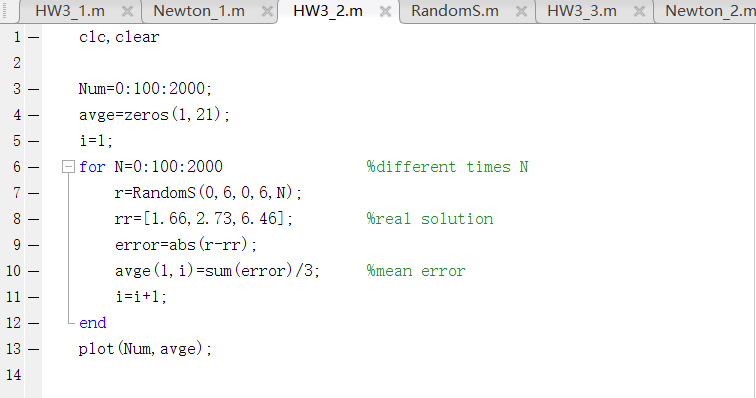
\includegraphics[scale=0.8]{figs/2_1.jpg}
    \caption{Main codes 2 in MATLAB}
\end{figure}

\newpage
\par I set a for loop to determine the answer after different N's iteration. 
Then I plot a graph which x-axis means $N$, and y-axis are 
{\bf the mean difference to the real answer} (which is $[1.616749,2.765987,6.46298]$). Seeing Figure 3. 
This solution is found since I let the iteration times to become $10^9$.

\par There is also some wave when $N\to \infty $ in Figure 4. 
That is because random search method is not accurate absolutely. 
There must be some points which is more optimal than founded point, since it takes random points. 

\par We can find that the mean difference is converging to 0 when N becoming larger and larger. 
{\bf So we can claim that there is a negetive ralationship between error and iteration times $N$.}

\begin{figure}[htbp]
    \centering
    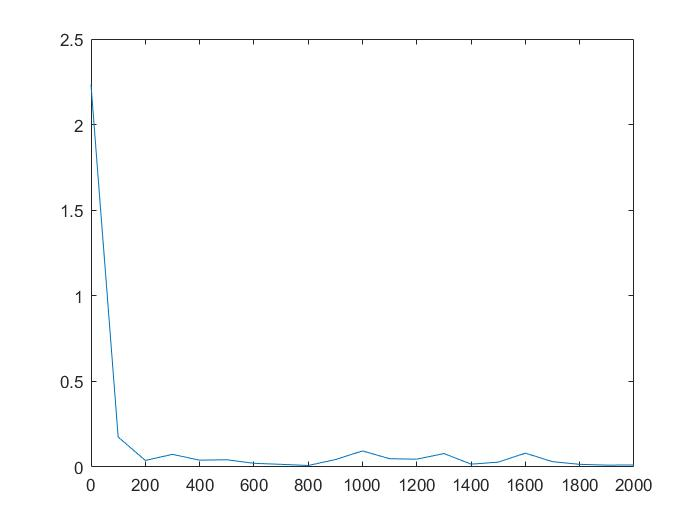
\includegraphics[scale=0.3]{figs/2_3.jpg}
    \caption{Graph of N and mean difference}
\end{figure}

\par Here is the codes to achieve random search method. 
\par The objective function is the function $z_m$ in {Figure 5.}.


\begin{figure}[htbp]
    \centering
    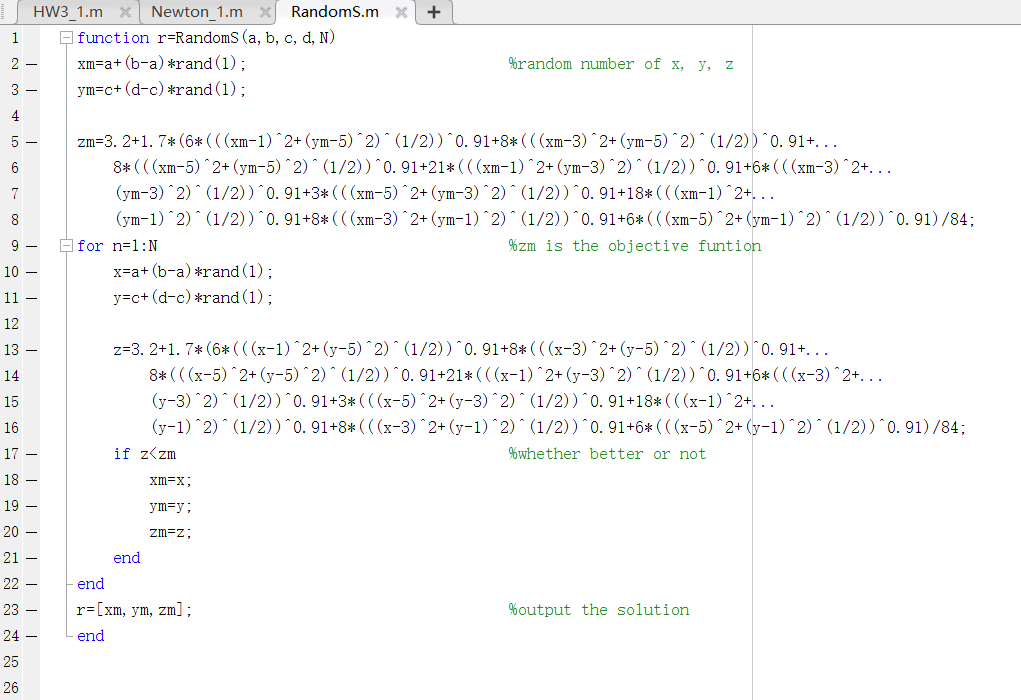
\includegraphics[scale=0.6]{figs/2_2.jpg}
    \caption{Function codes 2 in MATLAB}
\end{figure}


\newpage
\section*{question 3.}
\par In the example 2.2, there are 2 variables in order to solve. 
By using Multi-Variables Newton's Method we can finally find the best solution 
in $N$ times iteration, and this solution would have limited error to the real solution. 

\par Here is the codes in MATLAB\@. 

\begin{figure}[htbp]
    \centering
    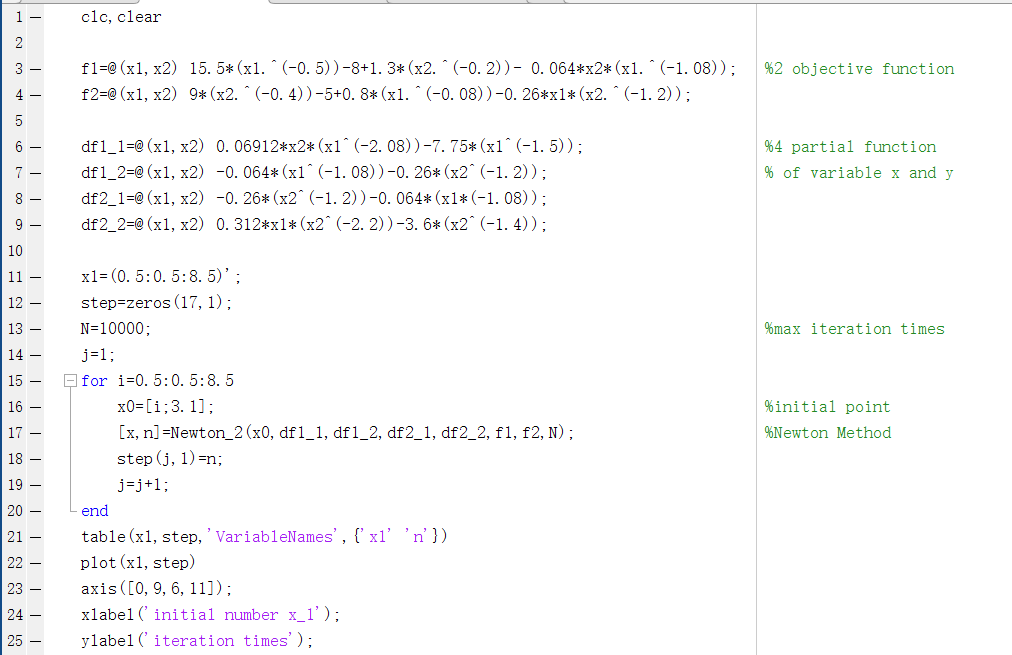
\includegraphics[scale=0.7]{figs/3_1.png}
    \caption{Main codes 3 in MATLAB}
\end{figure}

This program needs to input the partial function respected to variables $x_1$ and $x_2$. 
And $N$ is the max iteration times while $n$ is the real iteration times. 
In order to determine the relationship between initial point and iteration times, 
we must use different initial point. 
Obviously, we can find it between $x_1$ and $n$, and we can extend it to $x_2$. 
In my codes, I calculate $x_1$.

\newpage
\begin{figure}[htbp]
    \centering
    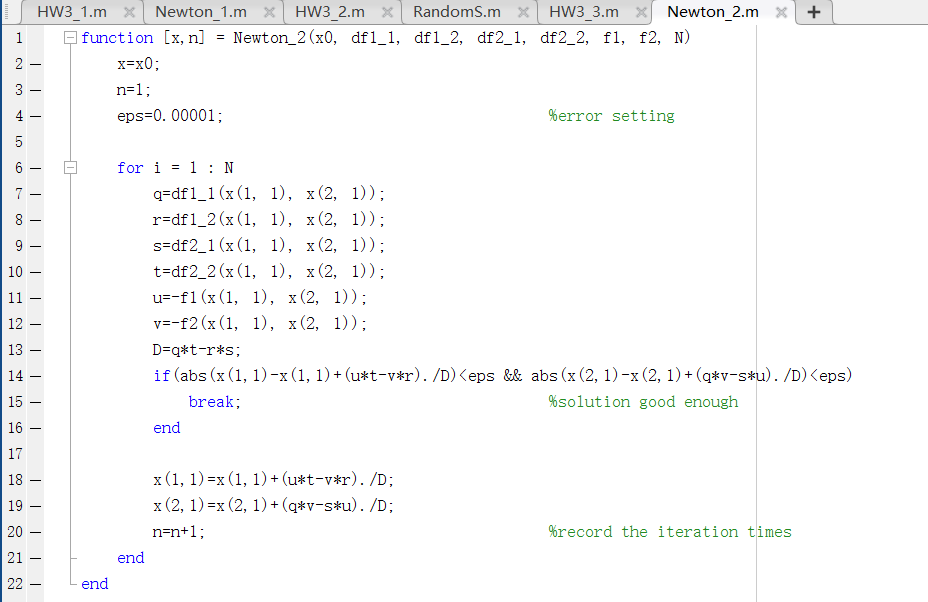
\includegraphics[scale=0.7]{figs/3_2.png}
    \caption{Function codes 3 in MATLAB}
\end{figure}

In this codes, I set the error requirment to be $eps =10^{-5}$. Seeing line 4.

\newpage
\par We want to find differnt initial point is how to effect the iteration times $n$. 
In the main codes I'd drawn a $x_1-n$ picture and a table which is 

\begin{figure}[htbp]
    \centering
    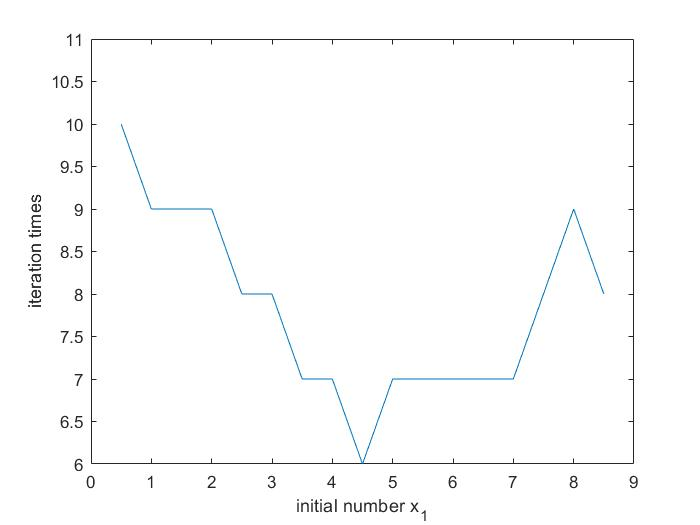
\includegraphics[scale=0.4]{figs/3_3.jpg}
    \caption{$x_1-n$ picture using by MATLAB}
\end{figure}

\begin{table}[htbp]
    \centering
    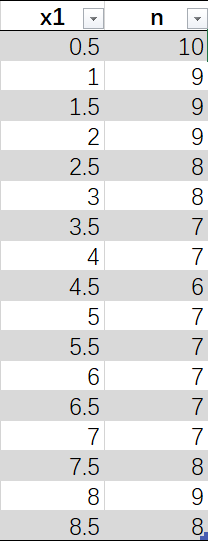
\includegraphics[scale=0.5]{figs/3_4.jpg}
    \caption{Sensitivity of initial point $x_1$ to iteration times $n$ for the question 3.}
\end{table}

\par Through the program we can find the optimal point is approaching to 
\begin{align*}
    x_1^* = 4.68959, x_2^* = 5.85199
\end{align*}


Then in the {Table 2}, we can find that if $x_2$ is a fixede initial point, the iteration times $n$ 
is going to be larger when $x_1$ is far away from the optimal solution $x_1^* = 4.68959$. 
Since the iteration times $n$ is going to lower between $x_1\in [0,8]$.
This trend also fixed for $x_2$. 
\par Also, there is a strange point when $x_1=8.5$, we can find that $n=8<9$.
After analysis I find that this leads to a wrong answer which is 
$x_1^* =6.36335, x_2^*=0.16817$. This is because the Hessian matrix is not positive definite. 
In other words, we need to find another matrix to approach Hessian matrix, then we can avoid this mistake. (Quasi-Newton Methods is better). 

{\bf So we can claim that iteration times $n$ become smaller when initial point is closer to the real solution. }







\end{document}